\ChapterImageStar[cap:caracterizacionGRID]{Caracterización del GRID}{./images/fondo.png}\label{cap:caracterizacionGRID}
\mbox{}\\
\noindent
El Grupo de Investigación en Redes, Información y Distribución (\GRID) de la Universidad del Quindío se enmarca en los objetivos misionales de la institución: educación, investigación y extensión. Uno del los intereses particulares del \GRID es ofrecer servicios tecnológicos avanzados a la comunidad académica, con énfasis en los estudiantes de Ingeniería de Sistemas y Computación, quienes encuentran en este grupo un espacio de formación e innovación en temas de infraestructura, ingeniería de software y tecnologías emergentes.\\
La caracterización del \GRID\ resulta esencial para comprender su estructura, capacidades y necesidades en relación con la expansión de un nuevo universo HTCondor. A continuación, se presenta un análisis de los diferentes aspectos que definen el contexto institucional y tecnológico del grupo.

\section{Análisis de stakeholders del GRID}
\noindent
Con el fin de identificar los actores internos y externos que influyen en el desarrollo de las actividades del grupo, se realizó un análisis de \textit{stakeholders}. Este ejercicio permitió reconocer los diferentes intereses, roles y niveles de influencia que cada actor tiene en relación con la expansión de un nuevo universo HTCondor. Los principales \textit{stakeholders} identificados incluyen: investigadores del grupo, estudiantes de pregrado y posgrado, docentes de la Facultad de Ingeniería, y en un nivel más amplio, la comunidad académica de la Universidad del Quindío.
\\
\noindent
La tablaef{tab:stakeholders} presenta el análisis de los principales interesados en la expansión de los universos HTCondor dentro del contexto institucional. Se identifican actores internos y externos, especificando su rol, el tipo de relación con el proyecto, el nivel de impacto esperado, así como su poder de influencia, interés y compromiso frente a la iniciativa.

El análisis de interesados revela una estructura compleja de actores con distintos niveles de influencia y compromiso frente al proyecto. El Grupo de Investigación GRID emerge como el interesado crítico, concentrando simultáneamente el mayor impacto, poder de influencia, interés y compromiso. Esta posición central le otorga un rol determinante como beneficiario principal y tomador de decisiones, lo que subraya la necesidad de mantener una comunicación estrecha y continua con este grupo para asegurar la alineación del proyecto con sus expectativas estratégicas y operativas.

Los docentes de Ingeniería de Sistemas y los investigadores locales y externos constituyen el segundo nivel de importancia, caracterizándose por un alto interés en la solución y un potencial significativo como usuarios finales. Aunque su poder de decisión es limitado, su adopción efectiva de la tecnología será fundamental para validar el éxito del proyecto. Este segmento requiere especial atención en términos de usabilidad, documentación y capacitación, dado que su compromiso está condicionado a la utilidad práctica y los beneficios tangibles que puedan obtener. La diferencia principal entre ambos grupos radica en que los investigadores externos representarían el segmento de usuarios más activo e intensivo de la infraestructura.

El Programa de Ingeniería de Sistemas y Computación desempeña un rol estratégico como facilitador institucional con alto poder de influencia, particularmente en la provisión de recursos y la posibilidad de escalar la solución hacia otros programas académicos. Sin embargo, su compromiso relativamente bajo sugiere que será necesario demostrar claramente el valor estratégico e institucional del proyecto para asegurar su respaldo sostenido. Por otro lado, los estudiantes de pregrado presentan bajo impacto, poder e interés debido a la naturaleza especializada de la computación distribuida en el contexto académico de pregrado, lo que los posiciona como beneficiarios secundarios que validarán la solución más por uso ocasional que por dependencia operativa.

Finalmente, la comunidad HTCondor y los investigadores en HTC y HPC representan un interesado externo con una relación simbiótica particular: aunque no tienen poder de decisión sobre el proyecto y su compromiso es bajo, su rol como proveedores de conocimiento técnico es de alto impacto. La documentación y experiencias generadas por el proyecto podrían contribuir al fortalecimiento del ecosistema HTCondor, creando un valor agregado que trasciende los objetivos locales del proyecto. Esta relación sugiere la conveniencia de establecer canales de comunicación con esta comunidad para compartir hallazgos y mejores prácticas.

\begin{table}[H]
	\centering
	\fontsize{7}{7}\selectfont % Cambia el primer número (9) al tamaño deseado, el segundo es el interlineado
	\setlength{\tabcolsep}{3pt} % reduce el espacio horizontal entre columnas
	\renewcommand{\arraystretch}{1.4} % espacio entre filas
	\begin{tabularx}{\textwidth}{%
		>{\raggedright\arraybackslash}p{1.7cm}  % Columna 1: Interesado
		>{\raggedright\arraybackslash}p{1.5cm}    % Columna 2: Rol
		>{\raggedright\arraybackslash}p{2.3cm}  % Columna 3: Relación
		>{\raggedright\arraybackslash}p{1.4cm}  % Columna 4: Impacto
		>{\raggedright\arraybackslash}p{2.0cm}  % Columna 5: Poder de influencia
		>{\raggedright\arraybackslash}p{2.5cm}    % Columna 6: Interés
		>{\raggedright\arraybackslash}p{2.0cm}} % Columna 7: Compromiso
		\toprule
		\textbf{Interesado}                              & \textbf{Rol}                               & \textbf{Relación}                                                                                                                                      & \textbf{Impacto} & \textbf{Poder de influencia}                                                                                            & \textbf{Interés}                                                                                                                          & \textbf{Compromiso}                                                                                \\
		\midrule
		Docentes de Ingeniería de Sistemas               & Usuarios clave                             & Utilizarán los entregables del proyecto en actividades de enseñanza e investigación                                                                    & Medio-Alto       & Medio, pueden proponer mejoras pero no tienen poder de decisión sobre la implementación                                 & Medio-Alto, requieren soliuciones tecnológicas para integrarlas en procesos académicos e investigativos                                   & Medio, condicionado a la utilidad práctica y aplicabilidad de la solución                          \\
		\midrule
		Estudiantes de Ingeniería de Sistemas            & Beneficiarios potenciales                  & Podrían utilizar la infraestructura en proyectos académicos y acceder a información sobre el estudio                                                   & Bajo             & Bajo, carecen de poder de decisión aunque su adopción validará la efectividad de la solución                            & Bajo, dado que la computación distribuida es un área especializada con uso poco frecuente en el contexto académico general                & Bajo                                                                                               \\
		\midrule
		Grupo de Investigación GRID                      & Beneficiario principal                     & Proporciona la infraestructura base, evalúa la solución propuesta y mide su impacto                                                                    & Alto             & Alto, tiene autoridad para decidir la adopción e implementación de la tecnología                                        & Alto, busca optimizar sus servicios y fortalecer su posicionamiento en el ámbito de la investigación y la colaboración interuniversitaria & Alto, la solución potenciará directamente sus capacidades de infraestructura                       \\
		\midrule
		Grupos de Investigación Locales y Externos       & Beneficiarios principales                  & Identificarían oportunidades significativas para potenciar sus líneas de investigación                                                                 & Medio            & Medio-Bajo, pueden influir mediante solicitudes específicas de funcionalidades o mejoras                                & Alto, la solución podría reducir significativamente los tiempos de procesamiento y obtención de resultados en sus proyectos               & Medio-Alto, conformarían uno de los segmentos principales de usuarios finales                      \\
		\midrule
		Programa de Ingeniería de Sistemas y Computación & Facilitador institucional                  & Puede proveer respaldo institucional, recursos y normativas que faciliten la adopción                                                                  & Alto             & Alto, posee autoridad para aprobar asignación de recursos e invitar a otros programas académicos a utilizar la solución & Medio, su interés se centra en aspectos institucionales y estratégicos más que operativos                                                 & Bajo-Medio, especialmente si la solución no impacta directamente sus procesos de gestión académica \\
		\midrule
		Comunidad HTCondor e investigadores en HTC y HPC & Proveedores y consumidores de conocimiento & Suministran documentación técnica esencial para la implementación y se benefician de la documentación generada a partir de la experiencia del proyecto & Alto             & Bajo, no participan en decisiones sobre el proyecto                                                                     & Bajo-Medio, la implementación exitosa fortalecería la adopción de HTCondor y ampliaría el impacto de la tecnología                        & Bajo, sujeto a la alineación de resultados con sus objetivos comunitarios                          \\
		\bottomrule
	\end{tabularx}
	\caption{Análisis de stakeholders}\label{tab:stakeholders}
\end{table}


\section{Priorización de stakeholders}
Una vez realizada la identificación de los \textit{stakeholders}, se emprendió un proceso de priorización para determinar cuáles poseen mayor impacto y poder de decisión en el proyecto. Esta clasificación resulta crucial para establecer estrategias de comunicación, gestión de expectativas y participación activa en la definición de requerimientos. De esta manera, se busca que los actores más influyentes en la toma de decisiones y en la adopción tecnológica sean atendidos de forma prioritaria, aumentando las probabilidades de éxito en la implementación.

\begin{figure}[H]
    \centering
    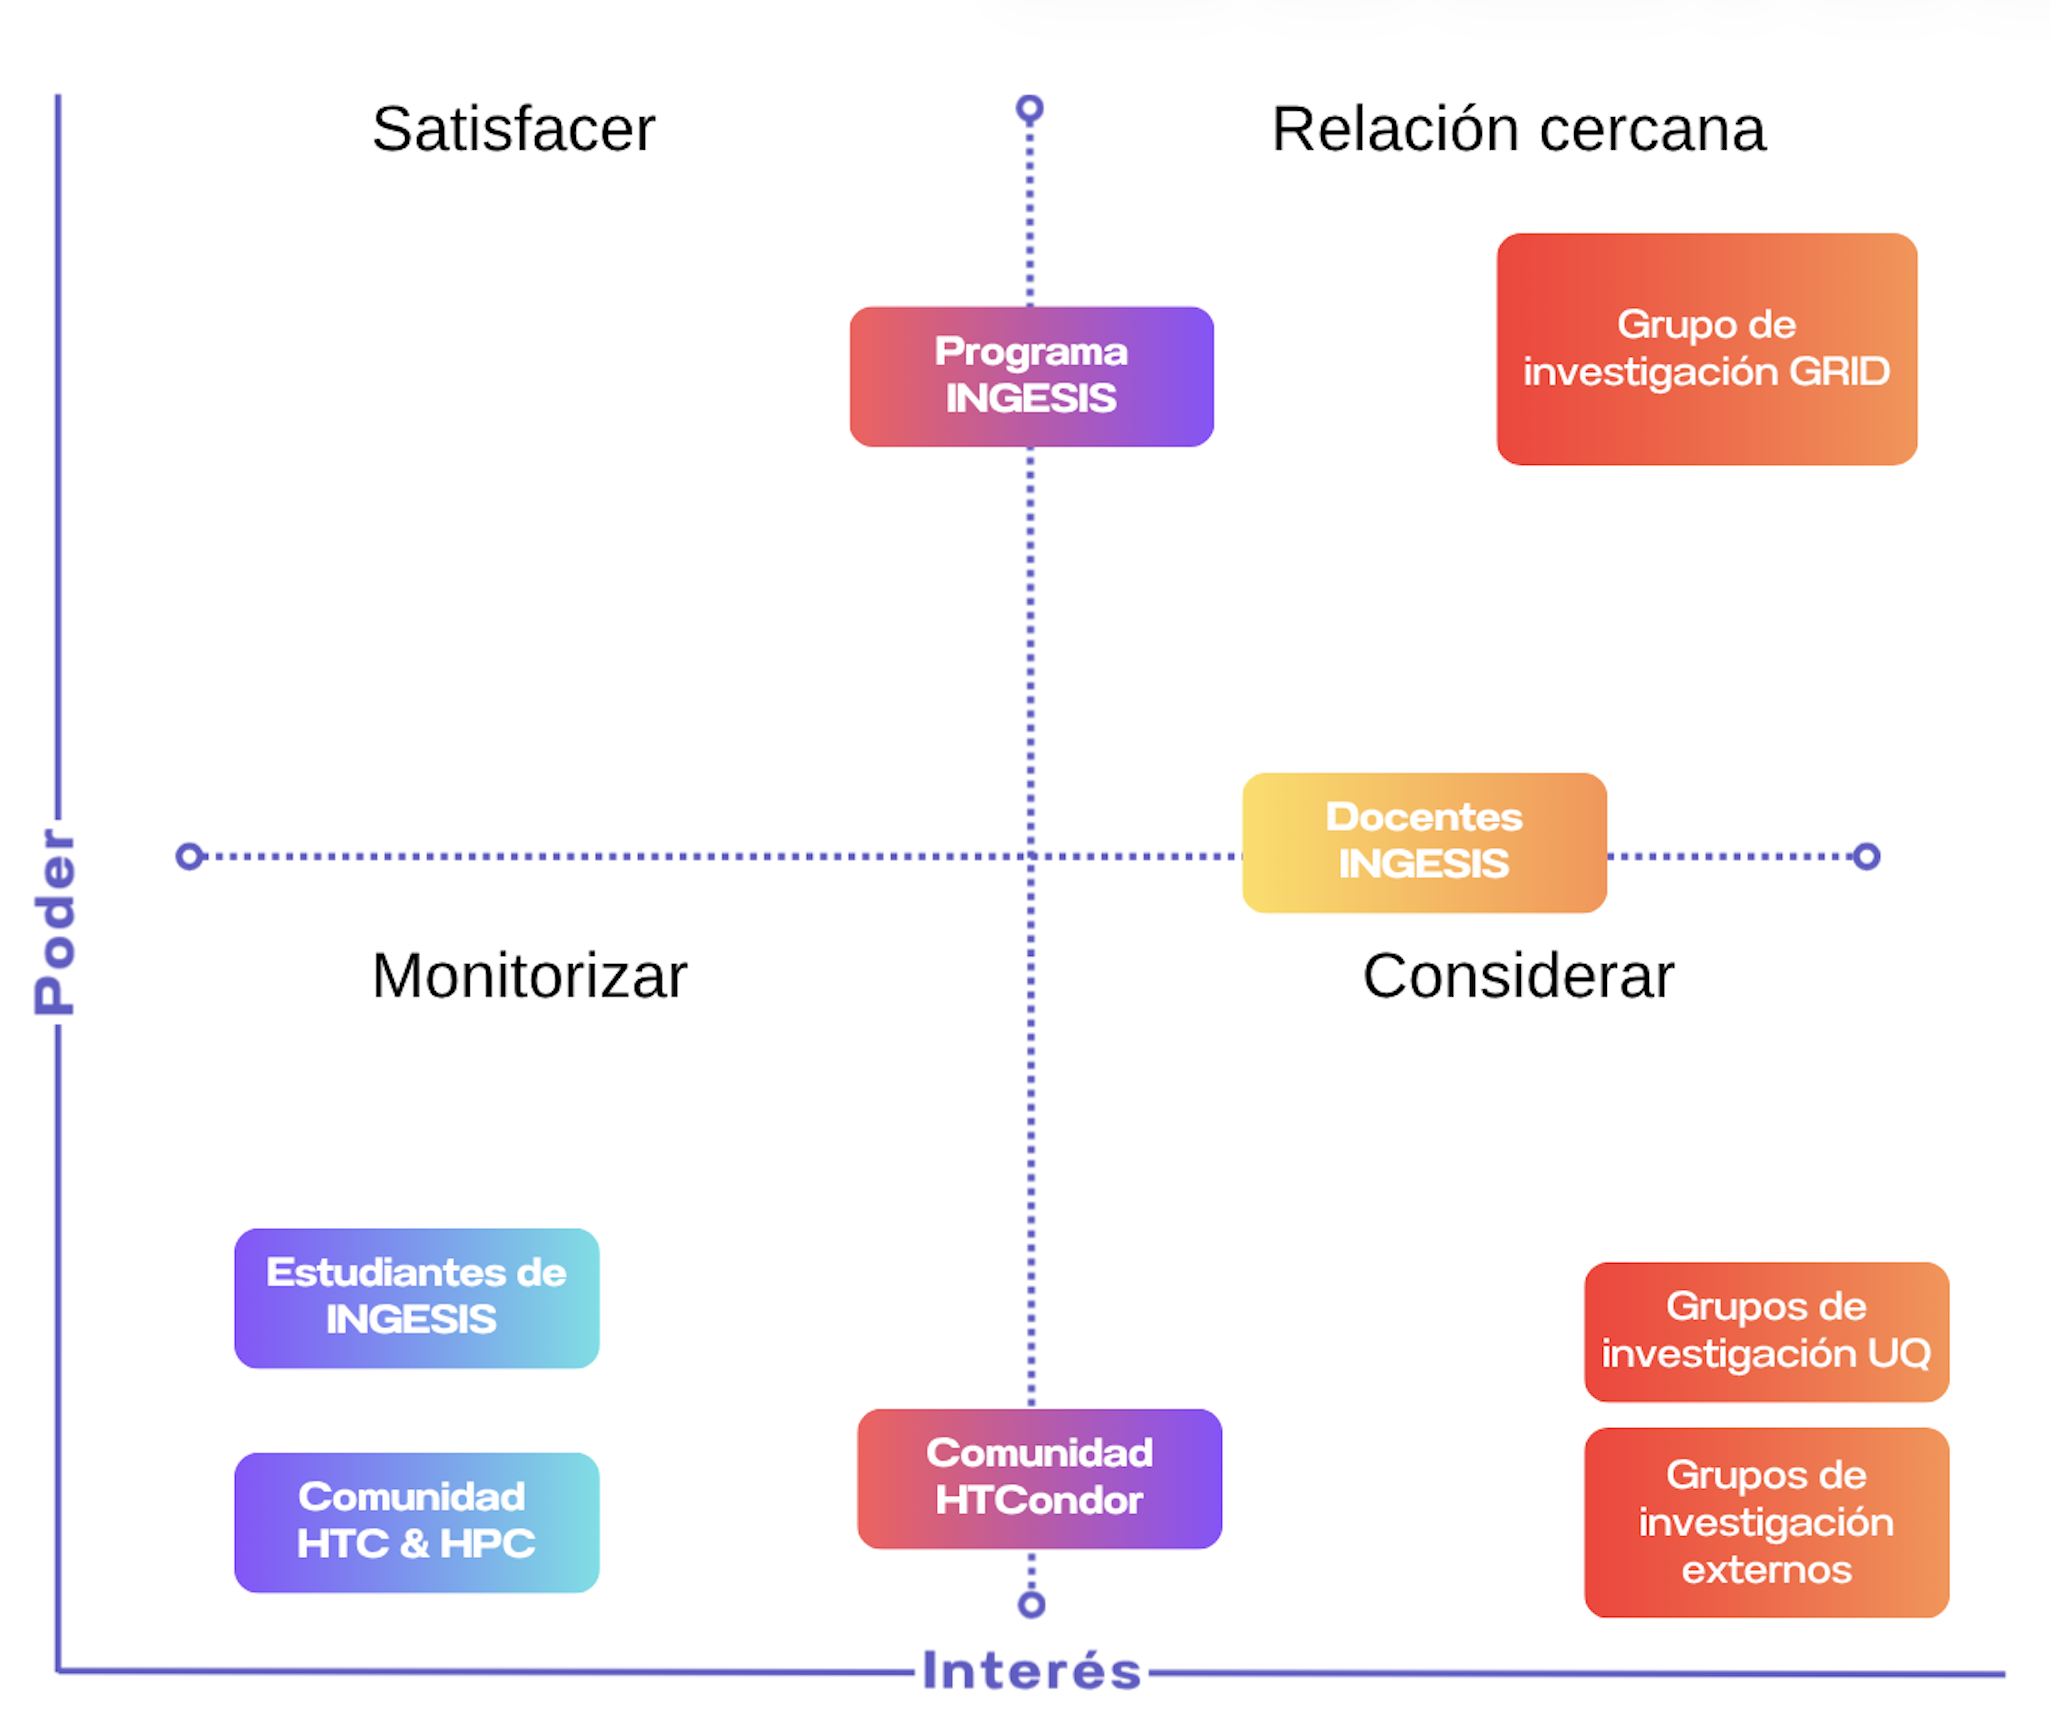
\includegraphics[width=\textwidth] {tablas-images/cp1/priorizacionStakeholders.png}
    \caption{Priorización de stakeholders del proyecto}\label{fig:tabla-priorizacion-stakeholders}
\end{figure}

\section{Integrantes y áreas de trabajo del GRID}
El \GRID\ está conformado por un equipo multidisciplinario de investigadores y profesionales que, desde sus diferentes áreas de experticia, contribuyen al avance en campos como computación de alto rendimiento, \textit{big data}, inteligencia artificial, redes de computadoras y desarrollo de software. A continuación, se presenta una lista de los integrantes actuales del grupo, junto con sus respectivas líneas de trabajo y áreas de especialización:
\begin{itemize}
	\item \href{https://scienti.minciencias.gov.co/cvlac/visualizador/generarCurriculoCv.do?cod_rh=0000210897}{\underline{{\textbf{Christian Andrés Candela Uribe}}}}: Microservicios, desarrollo de software, minería de datos, infraestructura TI.\@
	\item \href{https://scienti.minciencias.gov.co/cvlac/visualizador/generarCurriculoCv.do?cod_rh=0001383939}{\underline{{\textbf{Luis Eduardo Sepúlveda Rodríguez}}}}: Infraestructura de TI, HPC, computación paralela.
	\item \href{https://scienti.minciencias.gov.co/cvlac/visualizador/generarCurriculoCv.do?cod_rh=0001638854}{\underline{{\textbf{Carlos Andrés Flórez Villarraga}}}}: Programación y algoritmia, inteligencia artificial.
	\item \href{https://scienti.minciencias.gov.co/cvlac/visualizador/generarCurriculoCv.do?cod_rh=0001343801}{\underline{{\textbf{Carlos Eduardo Gómez Montoya}}}}: Redes, ingeniería de software, cloud computing.
	\item \href{https://scienti.minciencias.gov.co/cvlac/visualizador/generarCurriculoCv.do?cod_rh=0001398775}{\underline{{\textbf{Sergio Augusto Cardona Torres}}}}: Big data y análisis de datos, ingeniería de software, sistemas adaptativos, informática educativa.
	\item \href{https://scienti.minciencias.gov.co/cvlac/visualizador/generarCurriculoCv.do?cod_rh=0000193550}{\underline{{\textbf{Sonia Jaramillo Valbuena}}}}: Big data, electroquímica, inteligencia artificial.
	\item \href{https://scienti.minciencias.gov.co/cvlac/visualizador/generarCurriculoCv.do?cod_rh=0000283495}{\underline{{\textbf{Julián Esteban Gutiérrez Posada}}}}: Microservicios, desarrollo de software, minería de datos, infraestructura TI, HPC, computación paralela, redes, ingeniería de software.
\end{itemize}

La diversidad de líneas de trabajo de los integrantes fortalece la capacidad del grupo para abordar proyectos de carácter transversal y multidisciplinario, lo cual resulta particularmente relevante para el diseño e implementación de soluciones arquitectónicas soportadas en tecnologías de virtualización.

\section{Misión del GRID}
La misión del GRID es heredada de la Universidad del Quindío. A continuación se presenta la misión del GRID:\@

\begin{quote}
	\textit{La Universidad del Quindío contribuye a la transformación de la sociedad, mediante la formación integral desde el ser, el saber y el hacer, de líderes reflexivos y gestores del cambio; con estándares de calidad, a través de una oferta de formación en diferentes metodologías, que responda a una sociedad basada en el conocimiento; una investigación pertinente, que aporte a la solución de las problemáticas del desarrollo e integrada con la extensión y proyección social; educando en tiempos del posconflicto y de la consolidación de la paz, apoyada en una gestión creativa y con estándares de calidad.}
\end{quote}

A partir de esta misión, se identifican los siguientes pilares fundamentales:

\begin{itemize}
	\item \textbf{Docencia:} La Universidad del Quindío contribuye a la transformación de la sociedad, mediante la formación integral desde el ser, el saber y el hacer, de líderes reflexivos y gestores del cambio; con estándares de calidad, a través de una oferta de formación en diferentes metodologías, que responda a una sociedad basada en el conocimiento.

	\item \textbf{Investigación:} Una investigación pertinente, que aporte a la solución de las problemáticas del desarrollo e integrada con la extensión y proyección social.

	\item \textbf{Extensión y Desarrollo Social:} Apoyada en una gestión creativa y con estándares de calidad.

	\item \textbf{Responsabilidad Social:} Educando en tiempos del posconflicto y de la consolidación de la paz.
\end{itemize}

\section{Visión del GRID}
La misión de la Universidad del Quindío se complementa con su visión institucional, la cual también es adoptada por el \GRID. A continuación se presenta la visión del \GRID:\@

\begin{quote}
	\textit{En el año 2025, la Universidad del Quindío estará consolidada como una institución \textit{Pertinente --- Creativa --- Integradora}, acreditada de alta calidad, con reconocimiento nacional e internacional en sus procesos de formación a través de diferentes metodologías, de investigación, extensión, proyección y responsabilidad social.}
\end{quote}

A partir de esta visión, se destacan los siguientes enfoques estratégicos:

\begin{itemize}
	\item \textbf{Gestión:} La Universidad del Quindío estará consolidada como una institución \textit{Pertinente --- Creativa --- Integradora}.

	\item \textbf{Docencia:} Acreditada de alta calidad en sus procesos de formación a través de diferentes metodologías.

	\item \textbf{Investigación:} Consolidada como pertinente y de alta calidad en sus procesos de investigación.

	\item \textbf{Extensión y Desarrollo Social:} Procesos creativos e integradores en proyección social.

	\item \textbf{Responsabilidad Social:} Reconocimientos en sus procesos de responsabilidad social.
\end{itemize}

\section{Impacto del proyecto en el GRID}
La ampliación de la infraestructura HTCondor mediante la incorporación de un nuevo universo representa un impacto estratégico multidimensional para el Grupo de Investigación GRID. Este proyecto constituye un avance decisivo en la consolidación de una infraestructura de computación distribuida más amplia y capaz, lo que incrementa la competitividad del \GRID en el ámbito de la computación distribuida y de alta productividad. Además, esta expansión podría ayudar a fortalecer el posicionamiento del grupo como referente regional en tecnologías HTC y potenciar su capacidad para establecer colaboraciones interuniversitarias tanto a nivel nacional como internacional.


%%%%% ##############################################################################################################################
%%%%% ##############################################################################################################################
%%%%% ##############################################################################################################################
%%%%% #############################################################################################################################


\section{Caracterización de la infraestructura de computación distribuida del GRID}
\noindent
En la presente sección se especificarán las características técnicas actuales de la infraestructura de computación distribuida HTCondor del grupo \GRID.


% !TODO Verificar el conteo real de la máquinas.
\subsection{Clúster de máquinas Raspberry-Pi}\label{sec:cluster-raspberry}
\noindent

Actualmente, el grupo \GRID cuenta con un clúster compuesto por computadoras Raspberry Pi, distribuidas en nueve torres identificadas como \textbf{Torre 1} a \textbf{Torre 9}. Cada torre contiene siete equipos, con excepción de la Torre 1, que posee únicamente dos: uno opera como nodo maestro y el otro como nodo de envío de tareas. Los equipos restantes de las demás torres funcionan como nodos ejecutores.
\\
Si bien el \GRID posee nueve torres de equipos Raspberry-Pi, la torre novena se encuentra en funcionamiento. \\
%# Tablas de caracterización del GRID 

\begin{table}[h]
	\centering
	\begin{tabular}{|p{6cm}|p{8cm}|}
		\hline
		\multicolumn{2}{|c|}{\textbf{Características las máquinas Raspberry Pi del clúster HTCondor}} \\
		\hline
		Modelo                   & Raspberry Pi 3 Modelo B                                            \\
		\hline
		Versión                  & 1.2                                                                \\
		\hline
		CPU                      & ARMv7 de 1.2GHz                                                    \\
		\hline
		RAM                      & 1 GB                                                               \\
		\hline
		Cantidad de Procesadores & 4                                                                  \\
		\hline
		Sistema Operativo        & Raspbian GNU/Linux 9.1 (stretch) armv7l                            \\
		\hline
		Ubicación                & Oficina tercer piso                                                \\
		\hline
	\end{tabular}
	\caption{Especificaciones de la computadoras Raspberry Pi de GRID}
	\label{table:raspberries-pi-specs}
\end{table}





% Tabla con especificacioens de técnicas de las Raspberry-Pi
En la tabla \ref{table:raspberries-pi-specs} se pueden evidenciar las especificaciones técnicas de las máquinas disponibles para la infraestructura HTCondor del \GRID.
\\


%%#################################  FOTOS TORRES  #########################################
%Image de las Raspberry-Pi
\begin{figure}[H]
	\centering
	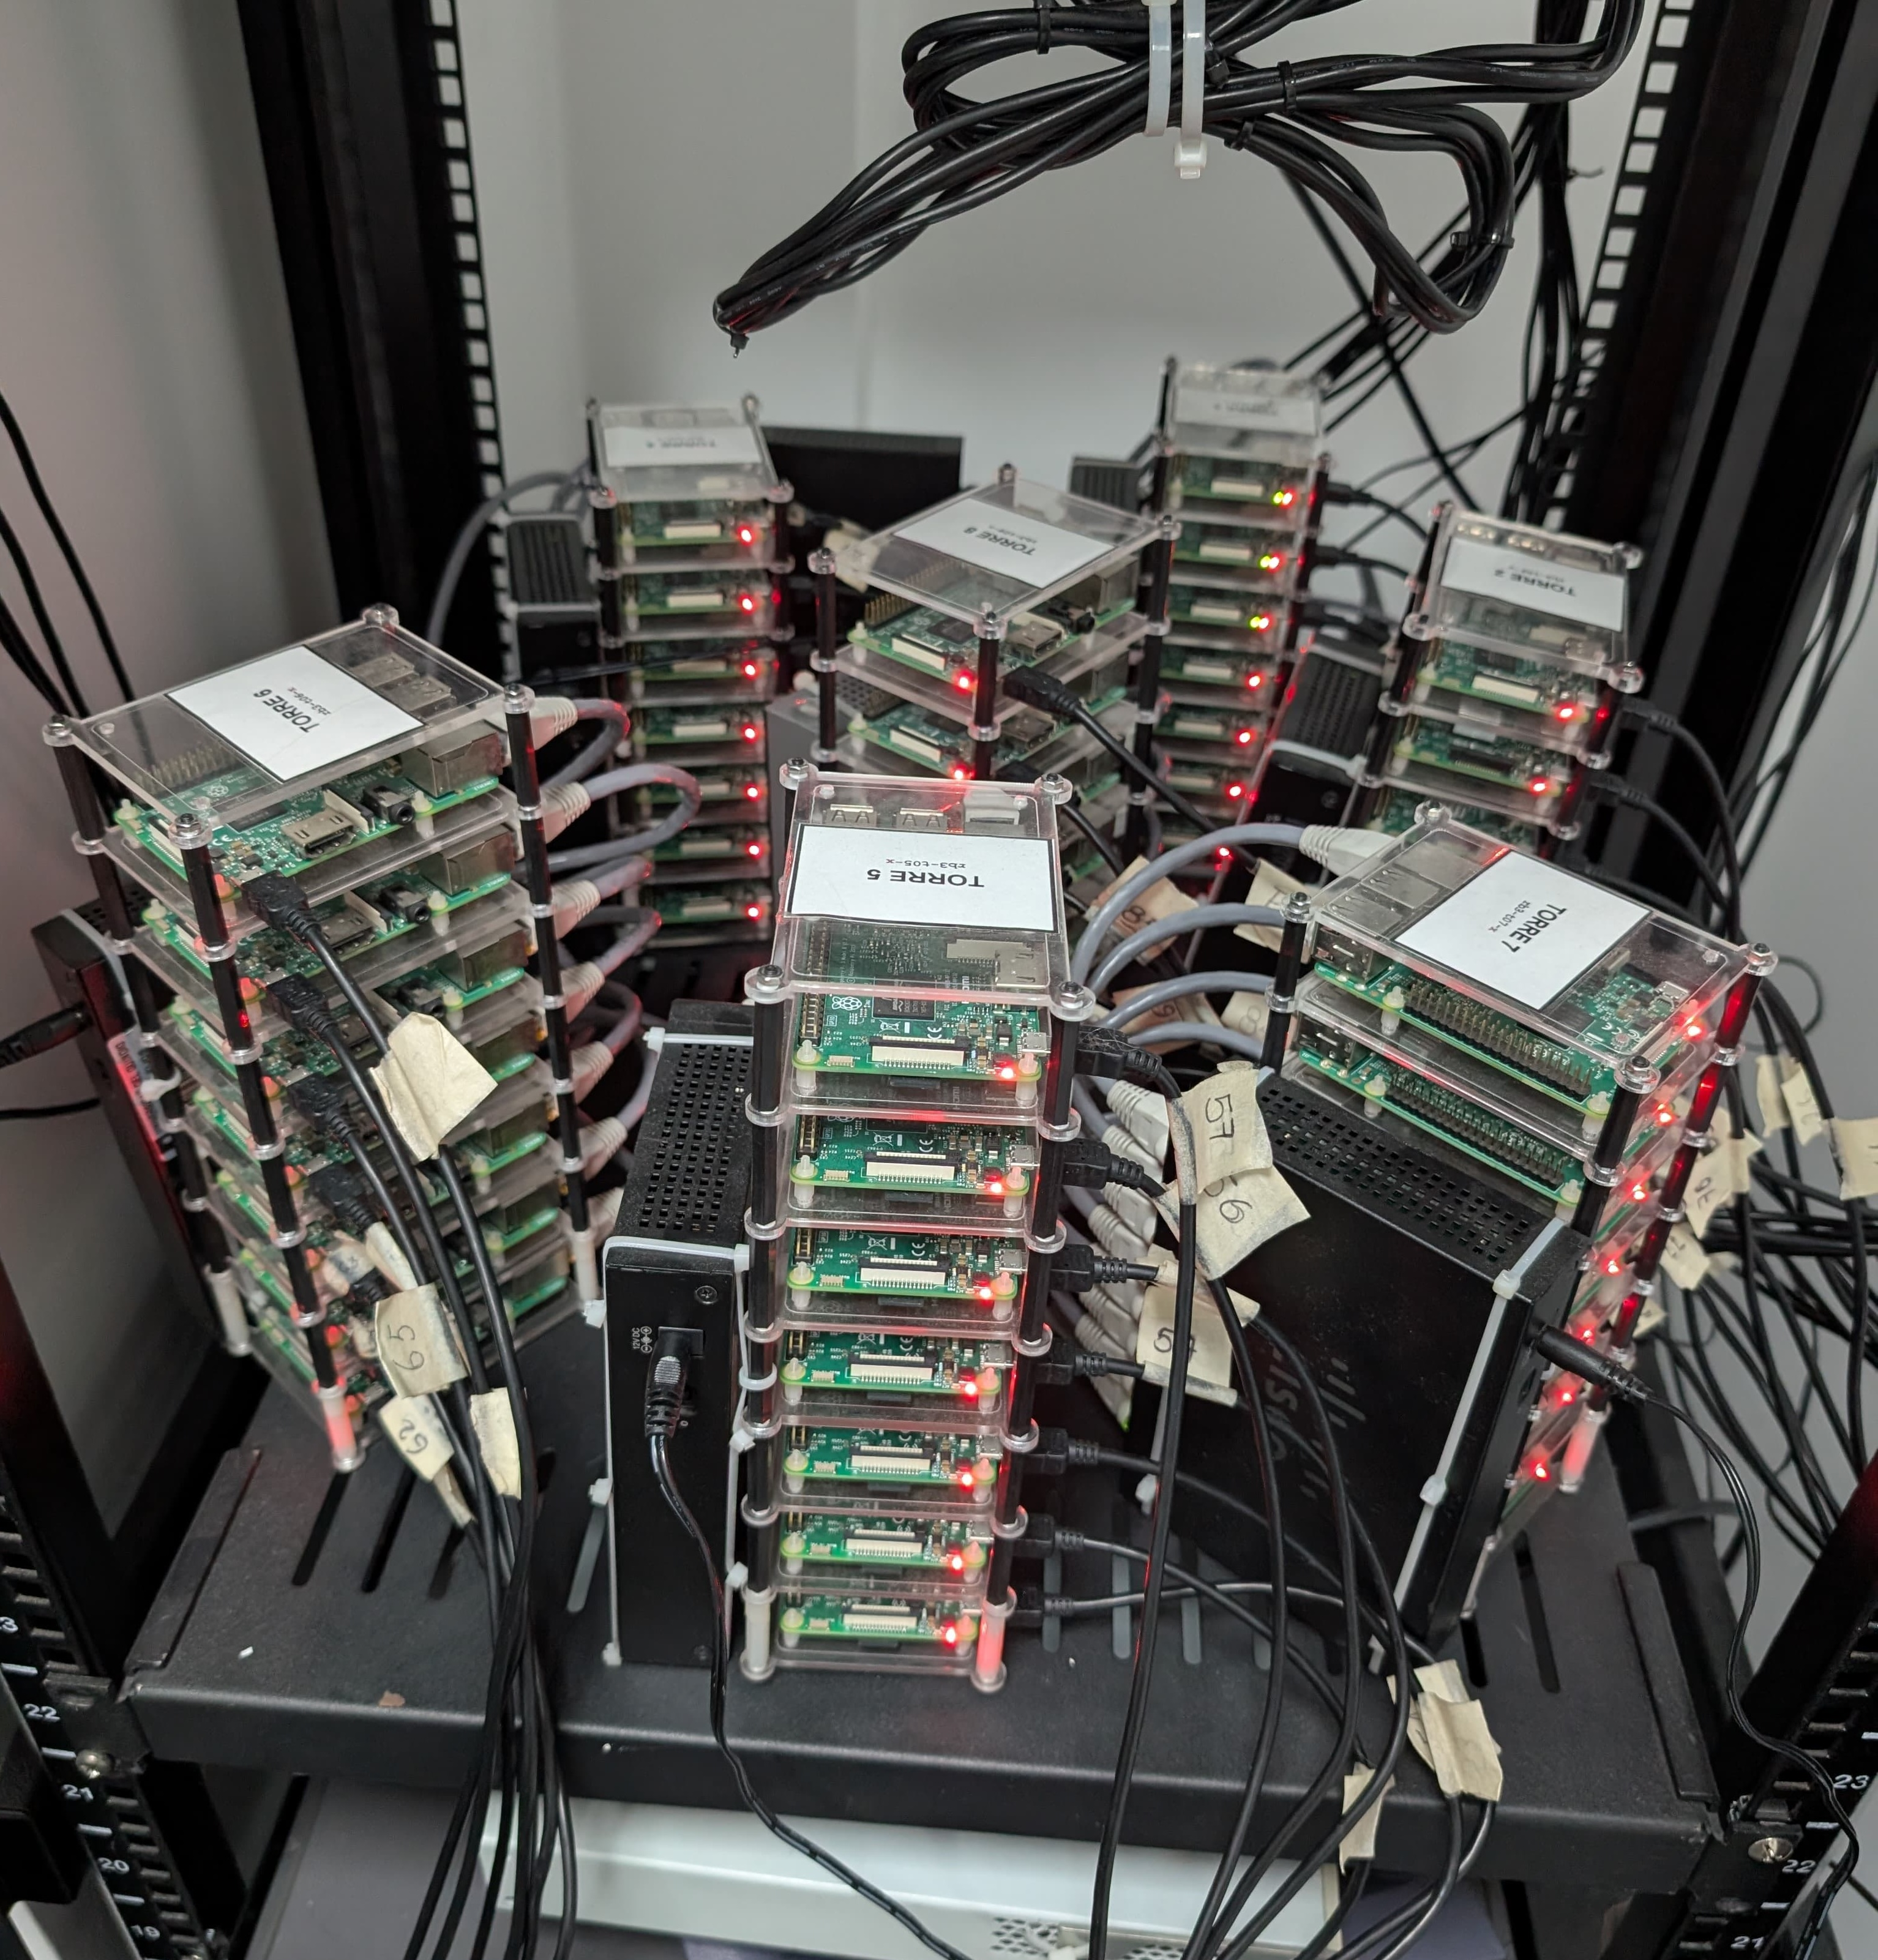
\includegraphics[scale=0.07]{tablas-images/raspberries/torres-raspberries.jpg}
	\caption{Vista general de las maquinas Raspberry-Pi}
	\label{fig:foto-torres-rasp}
\end{figure}


\noindent
En la figura \ref{fig:foto-torres-rasp} se muestra la imagen de las siete torres de Raspberry-Pi localizadas en la oficina del tercer piso de ingeniería. A continuación se muestran las demás torres individualmente.


%Torre BINARIA
\begin{figure}[H]
	\centering
	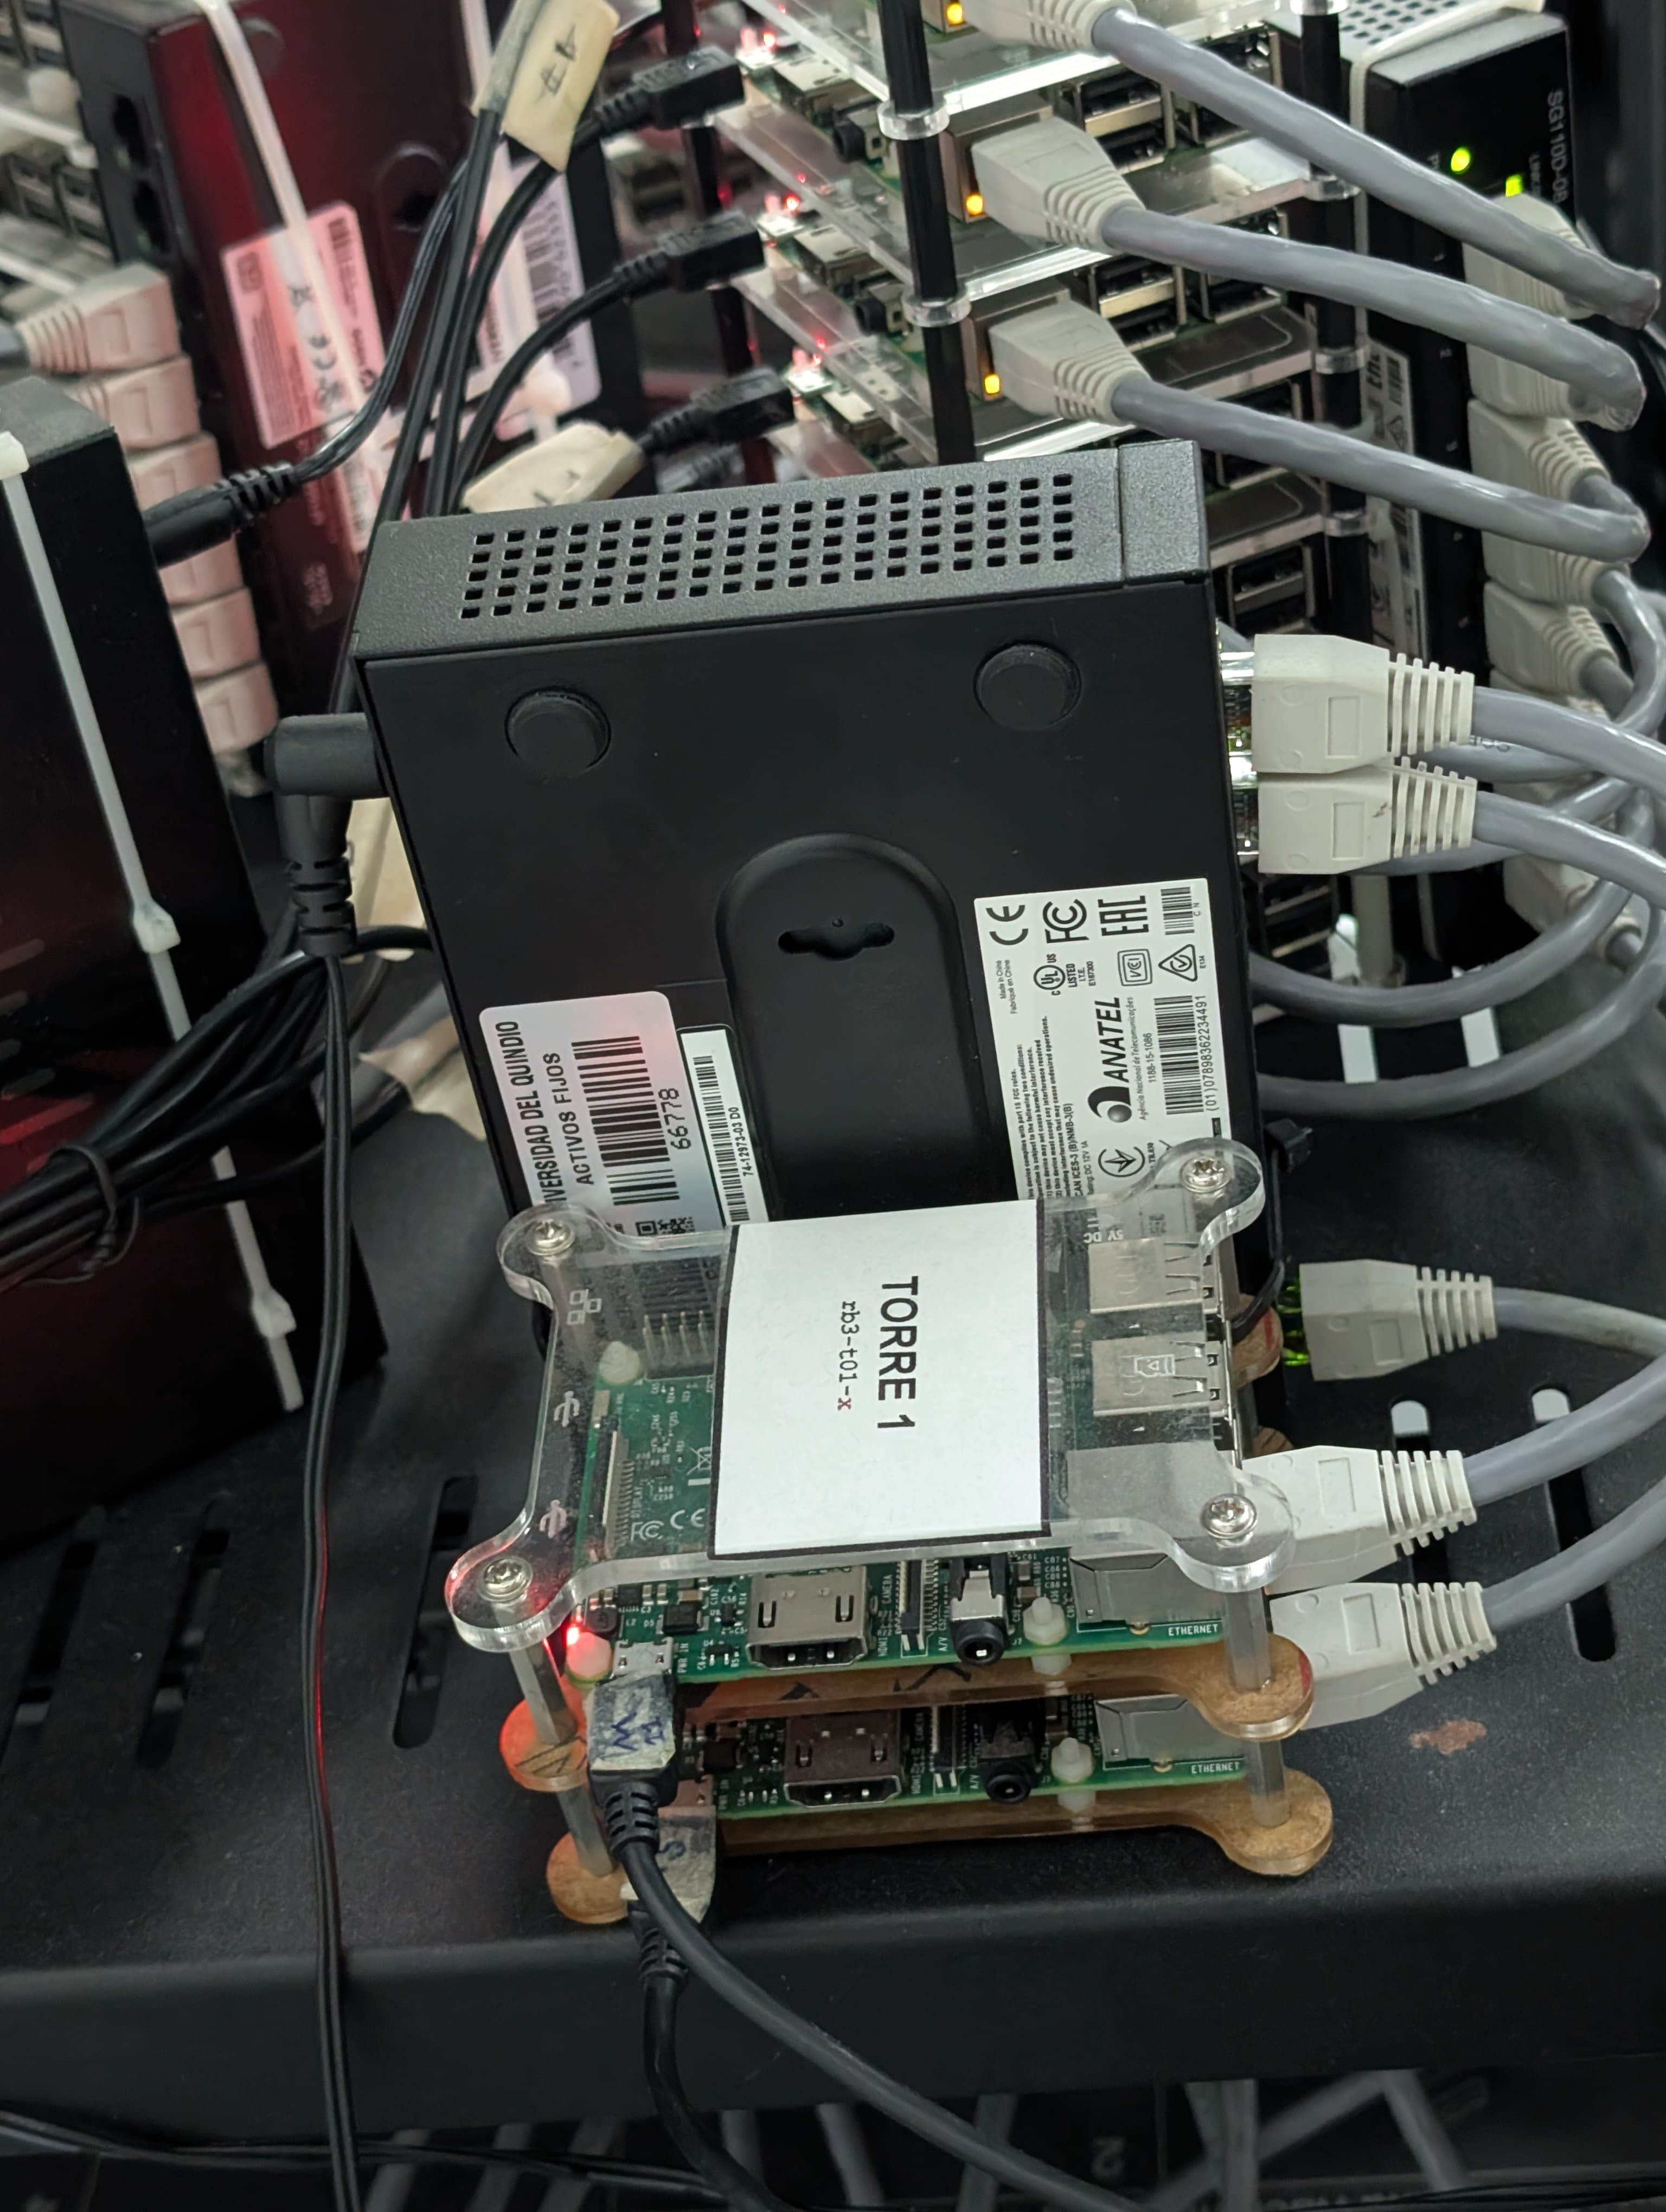
\includegraphics[scale=0.065]{tablas-images/raspberries/torre-binaria.jpeg}
	\caption{Vista general de las máquinas submit y master}
	\label{fig:foto-torre-binaria}
\end{figure}


% ####################################################################################################

\noindent
En la figura \ref{fig:foto-torre-binaria} se muestran las máquinas submit y master de clúster HTCondor.

\noindent
Como se puede evidenciar en las figuras \ref{fig:foto-torres-rasp} y \ref{fig:foto-torre-binaria}, cada máquina perteneciente a una torre está conectada a un switch. Las especificiones de dicho switch se mencionan en la tabla \ref{table:mini-switch}

% filepath: /Users/esteban/git-repos/ht-latex/tablas-images/raspberries/mini-switch.tex
%% Caracteristicas del switch al que están conectadas todas las maquinas HTCondor. 

\begin{table}[H]
	\centering
	\sffamily\scriptsize
	\setlength{\tabcolsep}{4pt}
	\renewcommand{\arraystretch}{1.3}
	\caption{Ficha técnica --- Switch Cisco SF100D-08}\label{table:mini-switch}
	\begin{tabular}{|p{0.25\textwidth}|p{0.6\textwidth}|p{0.12\textwidth}|}
		\hline
		\rowcolor{gray!15} \multicolumn{3}{|c|}{\textbf{DESCRIPCIÓN FÍSICA:} Switch de ocho puertos}                                                                                 \\ \hline

		\textbf{TIPO DE RECURSO:}                    & Switch       & \multirow{3}{*}{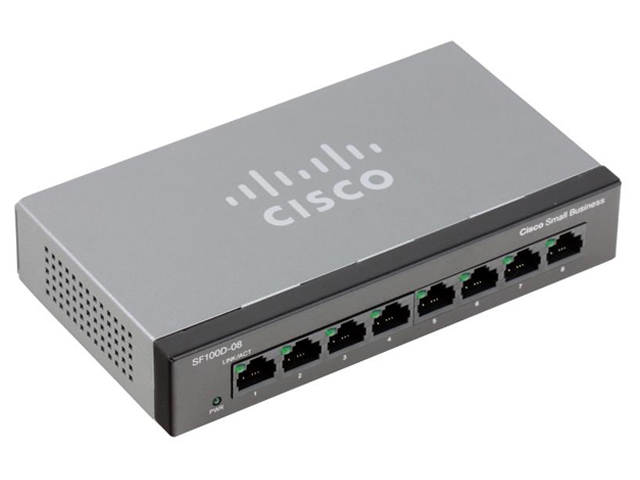
\includegraphics[width=\linewidth,keepaspectratio]{tablas-images/raspberries/mini-switch.jpg}} \\ \cline{1-2}
		\textbf{MODELO:}                             & SF100D-08 V2 &                                                                                                                \\ \cline{1-2}
		\textbf{MARCA:}                              & Cisco        &                                                                                                                \\ \hline

		\rowcolor{gray!15} \multicolumn{3}{|c|}{\textbf{ESPECIFICACIONES TÉCNICAS}}                                                                                                  \\ \hline

		\textbf{Rendimiento}                         &
		\begin{minipage}[t]{\linewidth}
			\vspace{2pt}
			• Capacidad de Conmutación: 1.6 Gbps \\
			• Capacidad de Reenvío: 1.4 mpps \\
			• Prevención de bloqueo HOL \\
			• Jumbo Frames: 9216 bytes
			\vspace{2pt}
		\end{minipage}      &                                                                                                                                         \\ \hline

		\textbf{Interfaces}                          &
		\begin{minipage}[t]{\linewidth}
			\vspace{2pt}
			• 8 puertos RJ-45 10BASE-T/100BASE-TX \\
			• Auto-negociación 10/100 Mbps \\
			• 4 colas de hardware (niveles de prioridad)
			\vspace{2pt}
		\end{minipage} &                                                                                                                                  \\ \hline

		\textbf{Estándares}                          &
		\begin{minipage}[t]{\linewidth}
			\vspace{2pt}
			• 802.3 10BASE-T Ethernet \\
			• 802.3u 100BASE-TX Fast Ethernet \\
			• 802.3x control de flujo \\
			• 802.1p prioridad \\
			• 802.3az Energy Efficient Ethernet
			\vspace{2pt}
		\end{minipage}         &                                                                                                                                           \\ \hline

		\textbf{Características Físicas}             &
		\begin{minipage}[t]{\linewidth}
			\vspace{2pt}
			• Alimentación: DC 12V, 500mA \\
			• Dimensiones: 140 × 33.35 × 140 mm \\
			• Peso: 0.38 kg \\
			• Montaje: Escritorio
			\vspace{2pt}
		\end{minipage}       &                                                                                                                                          \\ \hline

		\textbf{Certificaciones}                     &
		\begin{minipage}[t]{\linewidth}
			\vspace{2pt}
			UL (UL 60950), CSA (CSA 22.2), \\
			CE mark, FCC Part 15 Class A
			\vspace{2pt}
		\end{minipage}            &                                                                                                                                               \\ \hline

		\rowcolor{gray!15} \multicolumn{3}{|l|}{\textbf{PROPÓSITO:} Conexión de red para equipos del cluster HTCondor}                                                               \\ \hline
		\rowcolor{gray!15} \multicolumn{3}{|l|}{\textbf{OPORTUNIDAD DE USO:} Proyectos del \GRID}                                                                                    \\ \hline
		\multicolumn{3}{|p{0.97\textwidth}|}{\textbf{OBSERVACIONES:} Equipo de conectividad que proporciona comunicación entre todos los nodos del cluster HTCondor.}                \\ \hline
	\end{tabular}
\end{table}

\noindent
A su vez, los switch anteriores van conectados a otro switch. Este switch es el Cisco SG200-26. Sus especificaciones pueden verse en la tablas \ref{table:big-switch}

%% Características del switch principal del GRID

\begin{table}[H]
	\centering
	\sffamily\scriptsize
	\setlength{\tabcolsep}{4pt}
	\renewcommand{\arraystretch}{1.3}
	\caption{Ficha técnica --- Switch Cisco SG200-26}
	\label{table:big-switch}
	\begin{tabular}{|p{0.25\textwidth}|p{0.6\textwidth}|p{0.12\textwidth}|}
		\hline
		\rowcolor{gray!15} \multicolumn{3}{|c|}{\textbf{DESCRIPCIÓN FÍSICA:} Switch administrable de 26 puertos}                                                                                                                                 \\ \hline

		\textbf{TIPO DE RECURSO:}                     & Switch Gigabit administrable & \multirow{3}{*}{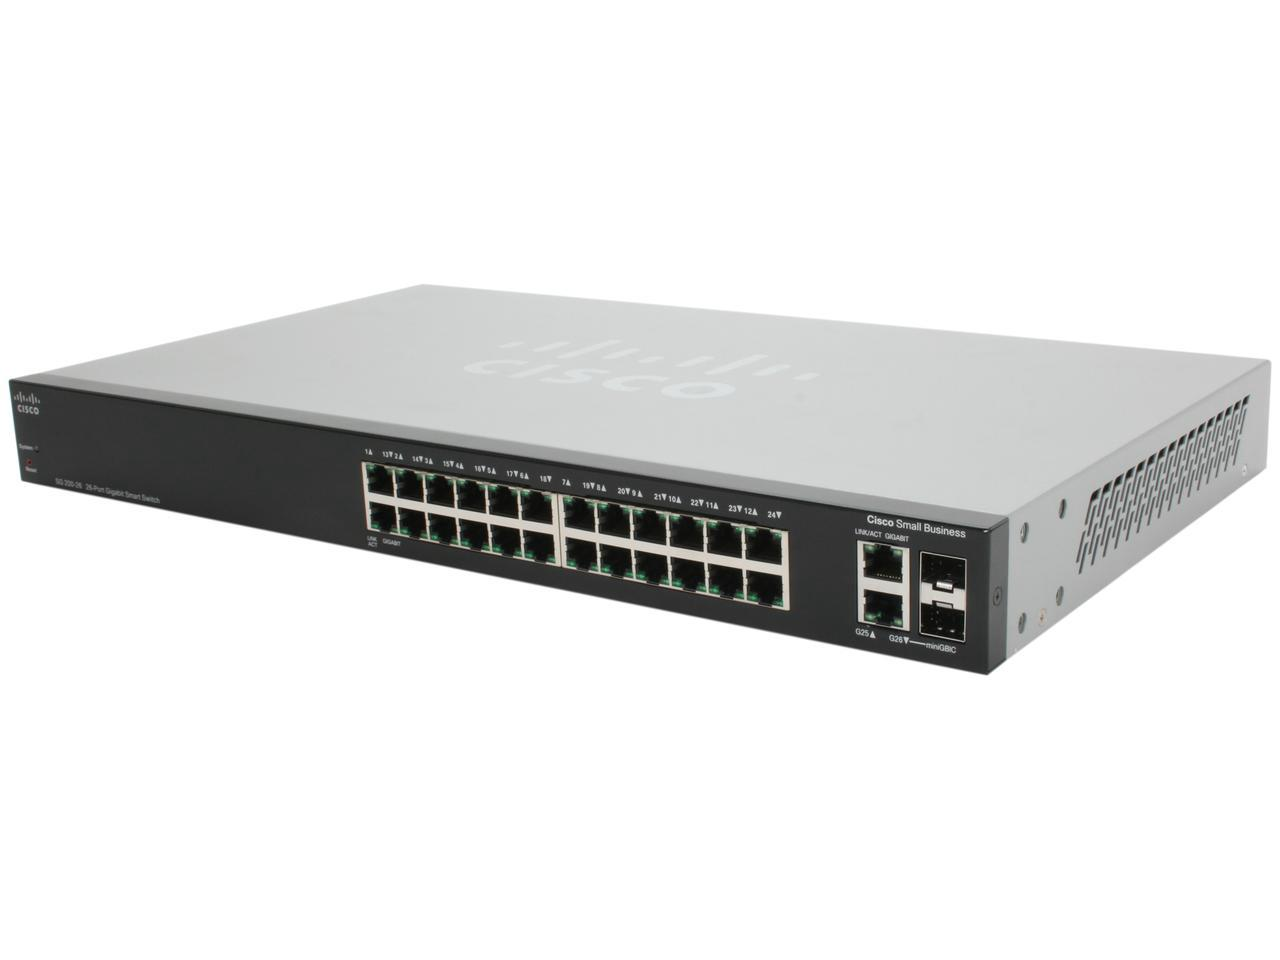
\includegraphics[width=\linewidth,keepaspectratio]{tablas-images/raspberries/big-switch.jpg}}                                             \\ \cline{1-2}
		\textbf{MODELO:}                              & SG200-26                     &                                                                                                                                                           \\ \cline{1-2}
		\textbf{MARCA:}                               & Cisco                        &                                                                                                                                                           \\ \hline

		\rowcolor{gray!15} \multicolumn{3}{|c|}{\textbf{ESPECIFICACIONES TÉCNICAS}}                                                                                                                                                              \\ \hline

		\textbf{Rendimiento}                          &
		\begin{minipage}[t]{\linewidth}
			\vspace{2pt}
			• Capacidad de Conmutación: 52 Gbps \\
			• Capacidad de Reenvío: 38.69 Mpps \\
			• Tabla de direcciones MAC: 8,000 entradas \\
			• Jumbo Frames: Soportado
			\vspace{2pt}
		\end{minipage} &                                                                                                                                                                                               \\ \hline

		\textbf{Interfaces}                           &
		\begin{minipage}[t]{\linewidth}
			\vspace{2pt}
			• 24 puertos RJ-45 10/100/1000 Mbps \\
			• 2 puertos combo Gigabit SFP \\
			• Auto-negociación y auto-MDI/MDIX \\
			• Soporte IEEE 802.3ad (Link Aggregation)
			\vspace{2pt}
		\end{minipage}     &                                                                                                                                                                                                 \\ \hline

		\textbf{Administración}                       &
		\begin{minipage}[t]{\linewidth}
			\vspace{2pt}
			• Interfaz web de administración \\
			• SNMP, RMON, HTTP, TFTP \\
			• Cisco Discovery Protocol \\
			• Auto SmartPorts \\
			• Soporte DHCP y BOOTP
			\vspace{2pt}
		\end{minipage}           &                                                                                                                                                                                                         \\ \hline

		\textbf{Características Avanzadas}            &
		\begin{minipage}[t]{\linewidth}
			\vspace{2pt}
			• VLAN support (IEEE 802.1Q) \\
			• Quality of Service (QoS) \\
			• IGMP/MLD Snooping \\
			• Spanning Tree (STP/RSTP) \\
			• IEEE 802.1x Authentication \\
			• Storm Control (Broadcast/Multicast/Unicast)
			\vspace{2pt}
		\end{minipage} &                                                                                                                                                                                             \\ \hline

		\textbf{Características Físicas}              &
		\begin{minipage}[t]{\linewidth}
			\vspace{2pt}
			• Alimentación: 100-240V AC, 50-60 Hz \\
			• Dimensiones: 439 × 257 × 43 mm \\
			• Peso: 3.3 kg (7.2 lbs) \\
			• Montaje: Rack 1U \\
			• Diseño sin ventiladores
			\vspace{2pt}
		\end{minipage}      &                                                                                                                                                                                                    \\ \hline

		\textbf{Memoria y Estándares}                 &
		\begin{minipage}[t]{\linewidth}
			\vspace{2pt}
			• Flash: 16 MB, RAM: 128 MB \\
			• IEEE 802.3/802.3u/802.3z/802.3ab \\
			• Certificaciones: UL 60950, FCC Part 15A \\
			• MTBF: 194,278 horas
			\vspace{2pt}
		\end{minipage}  &                                                                                                                                                                                                \\ \hline

		\rowcolor{gray!15} \multicolumn{3}{|l|}{\textbf{PROPÓSITO:} Switch principal para interconexión de infraestructura GRID}                                                                                                                 \\ \hline
		\rowcolor{gray!15} \multicolumn{3}{|l|}{\textbf{OPORTUNIDAD DE USO:} Backbone de red para servicios del \GRID}                                                                                                                           \\ \hline
		\multicolumn{3}{|p{0.97\textwidth}|}{\textbf{OBSERVACIONES:} Switch administrable de nivel empresarial que proporciona conectividad Gigabit con funciones avanzadas de gestión, VLAN, QoS y seguridad para la infraestructura del GRID.} \\ \hline
	\end{tabular}
\end{table}


\subsection{Ambientes de ejecución de la infraestructura HTCondor del \GRID}
\noindent{}
De acuerdo con la documentación oficial de HTCondor \citep{HTCondor-choosing-universe}, un universo se define como el ambiente de ejecución en el cual se lleva a cabo un trabajo. Al momento del desarrollo de la presente investigación, HTCondor contempla nueve universos disponibles: \textit{vanilla, grid, java, scheduler, local, parallel, vm, container} y \textit{docker}. Cada trabajo demanda, en función de sus características particulares, condiciones específicas de ejecución. A modo de ejemplo, un trabajo constituido por un programa desarrollado en lenguaje Java puede obtener ventajas significativas mediante la utilización del universo Java, lo cual facilita al usuario la configuración del ambiente de ejecución requerido.

Hasta el momento, la configuración de HTCondor del \GRID únicamente incorpora el universo vanilla, el cual está orientado a la ejecución no especializada de programas. En otras palabras, se trata de un universo de propósito general en el que los scripts de Shell han demostrado ser particularmente efectivos \citep{HTCondor-choosing-universe}.


\subsection{Servicios actuales de computación distribuida}
\noindent
Los servicios actuales del \GRID se orientan principalmente hacia la provisión de infraestructura de \TI, abarcando máquinas virtuales, soluciones de almacenamiento y configuración de redes. No obstante, la computación distribuida constituye un dominio especializado que demanda competencias técnicas avanzadas por parte de los usuarios. En consecuencia, si bien el grupo ha desarrollado capacidades en esta área, aún no se ha consolidado una oferta formal de servicios de computación distribuida de acceso público para la comunidad académica institucional.

% !TODO PREGUNTA PARA EL PROFE: Aquí hago una declaración temeraria sobre la universidad que neceisto confirmar
% Se han ofrecido servicios de computación identifica en el grupo grid que hayan estado disponibles para otros grupos o para 
% los mismo estudiantes de la universidad? 
%
\subsection{Servicios de computación distribuida esperados}
\noindent
Dado que no se ha establecido previamente un servicio de computación distribuida basado en HTCondor con acceso abierto para la comunidad educativa, resulta necesario identificar los potenciales beneficiarios que podrían aprovechar esta tecnología. Como señalan \cite{Wilson2016}, la computación se ha consolidado como un componente crítico del proceso científico en prácticamente todas las disciplinas, independientemente de su orientación hacia la experimentación o la simulación computacional. En este contexto, los usuarios que obtendrían mayor beneficio de la implementación de un servicio de computación distribuida serían aquellos cuyas actividades académicas o investigativas demanden capacidades de procesamiento intensivo para la obtención de resultados científicos. Por consiguiente, se estima que los principales beneficiarios de esta infraestructura serían tanto los estudiantes, quienes podrían fortalecer significativamente su proceso formativo mediante el acceso a una ambiente de computación distribuida, como los grupos de investigación institucionales, que verían ampliadas sus capacidades para desarrollar proyectos de mayor envergadura computacional. En la tabla \ref{table:servicio-htcondor} se especifica cómo podría verse un servicio de computación de alta productividad basado en HTCondor.

\begin{table}[H]
	\centering
	\sffamily\scriptsize
	\setlength{\tabcolsep}{4pt}
	\renewcommand{\arraystretch}{1.3}
	\caption{Caracterización del servicio de computación distribuida HTCondor esperado para el GRID}
	\label{table:servicio-htcondor}
	\begin{tabular}{|p{0.28\textwidth}|p{0.67\textwidth}|}
		\hline
		\rowcolor{gray!15} \multicolumn{2}{|c|}{\textbf{DESCRIPCIÓN GENERAL DEL SERVICIO}}                                                                                                                                                                                            \\ \hline

		\textbf{NOMBRE DEL SERVICIO}       & Servicio de Computación Distribuida HTCondor                                                                                                                                                                                             \\ \hline
		\textbf{TIPO DE SERVICIO}          & Servicio de educación, investigación y extensión universitaria                                                                                                                                                                           \\ \hline
		\textbf{HORARIO DE DISPONIBILIDAD} & 24/7 (Disponibilidad continua)                                                                                                                                                                                                           \\ \hline

		\rowcolor{gray!15} \multicolumn{2}{|c|}{\textbf{OBJETIVOS Y ALCANCE}}                                                                                                                                                                                                         \\ \hline

		\textbf{PROPÓSITO}                 &
		\begin{minipage}[t]{\linewidth}
			\vspace{2pt}
			Proveer infraestructura de computación de alta productividad (\HTC) para la ejecución de tareas computacionales intensivas y paralelas, facilitando el procesamiento distribuido de cargas de trabajo científicas y académicas
			\vspace{2pt}
		\end{minipage}                                                 \\ \hline

		\textbf{USUARIOS OBJETIVO}         &
		\begin{minipage}[t]{\linewidth}
			\vspace{2pt}
			• Estudiantes de pregrado y posgrado \\
			• Grupos de investigación institucionales \\
			• Docentes investigadores \\
			• Comunidad académica UQ
			\vspace{2pt}
		\end{minipage}                                                                                                                                                                                                                                     \\ \hline

		\rowcolor{gray!15} \multicolumn{2}{|c|}{\textbf{ESPECIFICACIONES TÉCNICAS}}                                                                                                                                                                                                   \\ \hline

		\textbf{RECURSOS DE HARDWARE}      &
		\begin{minipage}[t]{\linewidth}
			\vspace{2pt}
			• Clúster de máquinas Raspberry Pi \\
			• Máquinas virtuales especializadas \\
			• Infraestructura de red dedicada
			\vspace{2pt}
		\end{minipage}                                                                                                                                                                                                                                           \\ \hline

		\textbf{TECNOLOGÍAS}               &
		\begin{minipage}[t]{\linewidth}
			\vspace{2pt}
			• HTCondor (High Throughput Computing) \\
			• Sistemas de virtualización \\
			\vspace{2pt}
		\end{minipage}                                                                                                                                                                                                                                        \\ \hline

		\textbf{CAPACIDADES}               &
		\begin{minipage}[t]{\linewidth}
			\vspace{2pt}
			• Procesamiento paralelo de tareas independientes \\
			• Gestión automática de recursos \\
			• Balanceo de carga dinámico \\
			• Tolerancia a fallos
			\vspace{2pt}
		\end{minipage}                                                                                                                                                                                                                             \\ \hline

		\rowcolor{gray!15} \multicolumn{2}{|c|}{\textbf{APLICACIONES Y BENEFICIOS}}                                                                                                                                                                                                   \\ \hline

		\textbf{CASOS DE USO}              &
		\begin{minipage}[t]{\linewidth}
			\vspace{2pt}
			• Simulaciones científicas y modelado matemático \\
			• Procesamiento de datos masivos (Big Data) \\
			• Renderización de video y gráficos \\
			• Análisis bioinformático y genómico \\
			\vspace{2pt}
		\end{minipage}                                                                                                                                                                                                                              \\ \hline

		\textbf{IMPACTO ESPERADO}          &
		\begin{minipage}[t]{\linewidth}
			\vspace{2pt}
			• Fortalecimiento de capacidades investigativas \\
			• Democratización del acceso a recursos HTC \\
			• Apoyo a formación en computación distribuida \\
			• Incremento en productividad científica \\
			• Posicionamiento institucional en \HTC
			\vspace{2pt}
		\end{minipage}                                                                                                                                                                                                                               \\ \hline

		\rowcolor{gray!15} \multicolumn{2}{|l|}{\textbf{CONTRIBUCIÓN:} Expansión de universos HTCondor para mayor versatilidad}                                                                                                                                                       \\ \hline
		\multicolumn{2}{|p{0.95\textwidth}|}{\textbf{OBSERVACIONES:} Servicio orientado a democratizar el acceso a recursos de computación de alto rendimiento para la comunidad académica, fortaleciendo las capacidades investigativas y formativas de la Universidad del Quindío.} \\ \hline
	\end{tabular}
\end{table}
\section{Descripción de la oportunidad}
\noindent
La implementación de un nuevo universo HTCondor en la infraestructura del grupo GRID representa una oportunidad estratégica de considerable valor tanto para la comunidad académica de la Universidad del Quindío como para los grupos de investigación locales y externos. En primer lugar, esta ampliación abrirá el paso para que diversos grupos de investigación de la institución accedan a capacidades computacionales especializadas más diversas, democratizando así el uso de tecnologías de computación distribuida para disciplinas que requieren procesamiento intensivo de datos, tales como la bioinformática, el análisis de big data, el aprendizaje profundo y la simulación científica. En segundo lugar, desde una perspectiva formativa, la incorporación de este nuevo universo constituye una oportunidad invaluable para que los estudiantes de pregrado y posgrado adquieran competencias prácticas en computación de alto rendimiento (\HTC), un campo con limitada documentación y experiencias de implementación documentadas en el contexto colombiano. Adicionalmente, esta iniciativa ayudaría al posicionamiento del \GRID como un referente en computación distribuida a nivel nacional, facilitando la colaboración interinstitucional y el desarrollo de proyectos conjuntos con otras universidades e instituciones de investigación. Finalmente, la consolidación de una infraestructura HTCondor más robusta y versátil contribuye directamente a la competitividad investigativa de la Universidad del Quindío, optimizando el aprovechamiento de recursos computacionales disponibles y generando capacidades técnicas diferenciadas que pueden traducirse en publicaciones científicas, proyectos de mayor envergadura y fortalecimiento de las líneas de investigación institucionales.


\section{Resumen de la entrevista con el cliente}

Para comprender mejor las necesidades y expectativas del \GRID\, se realizó una entrevista con el cliente.

%!TODO  Entrevista
\begin{itemize}
	\item \textbf{Entrevistado:} Luis Eduardo Sepúlveda Rodríguez
	\item \textbf{Fecha:} XXXXXXXXX
	\item \textbf{Duración:} XXXXXXXXXXX
	\item \textbf{Link:} \href{https://drive.google.com}{click aquí}
	\item \textbf{Asistentes:} Juan Esteban Castaño Osma, Juan Esteban Parra Parra
\end{itemize}
